% El bus de features: de dónde sale cada ranura y quién lo consume.
% Fuente: modulos/mca/rtl/mca_publish.sv (armado) y mca_top.sv (consumidores).
% Compilar:   pdflatex bus_features.tex && pdftocairo -svg bus_features.pdf bus_features.svg
\documentclass[border=0pt,tikz]{standalone}
\usepackage[utf8]{inputenc}
\usepackage[T1]{fontenc}
\usepackage{lmodern}
\usepackage[none]{hyphenat}
% Estilo común de las figuras TikZ (panoramas y diagramas de bloques).
%
% Cada figura lo incluye con \input{../../figuras/estilo_tikz.tex} (las figuras
% viven en docs/<módulo>/figuras/). Un solo lugar para la paleta, los estilos de
% bloque y el formato de los parámetros: si cambia algo acá, cambia en todas.
%
% La paleta es la misma de docs/figuras/estilo_svg.py y de PALETA en
% modulos/mk/datasheet.py; si se toca un color, se toca en los tres.
%
% Requiere: \usepackage{tikz} (lo da la clase standalone con la opción tikz).

\usetikzlibrary{arrows.meta,positioning,calc,fit,backgrounds,shapes.multipart,
                decorations.markings,shadows}

% ---------------------------------------------------------------- colores ---
\definecolor{azul}{RGB}{108,172,228}      % acondicionamiento
\definecolor{verde}{RGB}{110,214,142}     % captura / histogramas en BRAM
\definecolor{amarillo}{RGB}{252,232,160}  % trigger
\definecolor{naranja}{RGB}{252,206,160}   % camino a DDR
\definecolor{grisr}{RGB}{226,226,226}     % compartido / infraestructura
\definecolor{rojo}{RGB}{240,128,128}      % bus del sistema

% ---------------------------------------------------------------- estilos ---
\tikzset{
  >={Stealth[length=2.4mm,width=1.8mm]},
  % fondo blanco siempre: el SVG se ve igual en modo claro y oscuro
  fondo/.style   = {show background rectangle, inner frame sep=8pt,
                    background rectangle/.style={fill=white, draw=none}},
  bloque/.style  = {draw=black, line width=0.6pt, rounded corners=2pt,
                    align=center, text width=2.2cm, minimum height=1.15cm,
                    inner sep=2pt, font=\scriptsize, fill=#1},
  datos/.style   = {bloque=azul!35},
  trig/.style    = {bloque=amarillo},
  captura/.style = {bloque=verde!55},
  ddr/.style     = {bloque=naranja!70},
  comp/.style    = {bloque=grisr},
  bus/.style     = {bloque=rojo!45},
  % lógica escrita dentro del módulo, sin submódulo propio
  etapa/.style   = {bloque=#1, line width=0.5pt},
  etapa/.default = verde!20,
  % lo que el bitstream no trae (atado a cero, stub, salida muda)
  mudo/.style    = {bloque=white, draw=black!45, dashed, text=black!55},
  %
  % BLOQUE CON PARÁMETROS, en el formato del datasheet: el encabezado lleva el
  % nombre y los parámetros con que lo instancia el padre (NOMBRE=valor, en
  % monoespaciada, uno por línea); el cuerpo, más claro, lo que hace.
  %   \node[datos, param={azul!35}{azul!12}] {\blk{nombre}{} \prm{A=1\\B=2}
  %                                            \nodepart{two} función};
  param/.style 2 args = {rectangle split, rectangle split parts=2,
                         rectangle split part fill={#1, #2}},
  %
  flujo/.style   = {->, line width=0.8pt},
  ctrl/.style    = {->, line width=0.6pt, black!65},
  % la línea que pasa por encima en un cruce: un halo blanco la separa
  cruce/.style   = {preaction={draw=white, line width=3.4pt, -}},
  % marca de ancho de bus: barra oblicua a mitad de la flecha, con el número
  % encima. \draw[flujo, ancho=14] ...; para otra posición, ancho en=0.3.
  ancho/.style   = {decoration={markings, mark=at position \anchopos with {
                      \draw[line width=0.6pt, -] (-0.1,-0.14) -- (0.1,0.14);
                      \node[font=\scriptsize, above=1.5pt] {#1};}},
                    postaction={decorate}},
  % la misma marca en una flecha vertical: el número va a la derecha
  anchov/.style  = {decoration={markings, mark=at position \anchopos with {
                      \draw[line width=0.6pt, -] (-0.14,-0.1) -- (0.14,0.1);
                      \node[font=\scriptsize, right=3pt] {#1};}},
                    postaction={decorate}},
  ancho en/.code = {\def\anchopos{#1}},
  sen/.style     = {font=\scriptsize\ttfamily, inner sep=1.5pt},
  nodo/.style    = {font=\tiny\ttfamily, inner sep=1pt, black!75},
  pin/.style     = {font=\scriptsize, align=center, inner sep=1pt},
  grupo/.style   = {draw=black!55, dashed, line width=0.7pt, rounded corners=4pt},
  canal/.style   = {grupo},
  contenedor/.style = {draw=black!80, line width=1.0pt, rounded corners=6pt},
  % marca numerada: cada número es una fila de la tabla del documento
  marca/.style   = {circle, fill=black, text=white, font=\scriptsize\bfseries,
                    inner sep=0pt, minimum size=4.3mm},
  %
  % DECISIONES (docs/mca/vista_general_mca.md). Cada opción es un bloque, todas
  % entran a un mux (\muxdec, abajo) y el registro que elige entra por abajo.
  % la opción que trae el reset (el comportamiento histórico): borde doble
  defecto/.style = {double=white, double distance=0.8pt, line width=0.45pt},
  % rótulo de la decisión, el mismo Dn del panorama y del documento
  decision/.style = {circle, fill=black, text=white, font=\small\bfseries,
                     inner sep=0pt, minimum size=7mm},
  %
  % LÓGICA (docs/mca/figuras/contabilidad/ y los detalles de las decisiones)
  % registro: caja gris con el triángulo de reloj en el borde de abajo
  registro/.style = {draw=black, line width=0.6pt, fill=grisr, align=center,
                     font=\scriptsize, inner sep=2pt, minimum width=#1,
                     minimum height=0.85cm,
                     path picture={\draw[line width=0.5pt]
                       ([xshift=-1.1mm]path picture bounding box.south) --
                       ([yshift=1.6mm]path picture bounding box.south) --
                       ([xshift=1.1mm]path picture bounding box.south);}},
  registro/.default = 0.8cm,
  % condición de una cadena if / else-if: "sí" sale a la derecha, "no" abajo
  pregunta/.style = {draw=black, line width=0.5pt, rounded corners=7pt,
                     fill=white, font=\scriptsize\ttfamily, align=center,
                     inner sep=2.5pt, minimum height=0.62cm, text width=#1},
  pregunta/.default = 1.9cm,
  si/.style      = {font=\tiny, inner sep=1pt, above, pos=0.12},
  no/.style      = {font=\tiny, inner sep=1pt, left, pos=0.45},
  %
  titulo/.style  = {anchor=north west, font=\small, inner sep=4pt, align=left},
  rotulo/.style  = {anchor=north west, font=\scriptsize\itshape, black!70,
                    inner sep=2pt, align=left},
}

% submódulo: nombre en monoespaciada; lógica propia: nombre en romana
\newcommand{\blk}[2]{{\ttfamily\bfseries #1}\\[1pt]#2}
\newcommand{\etq}[2]{{\bfseries #1}\\[1pt]#2}
\newcommand{\punto}[1]{\fill (#1) circle (1.3pt);}

% Parámetros en el formato del datasheet: NOMBRE=valor en monoespaciada, una
% entrada por celda, hasta cuatro columnas. Una columna: \prm{A=1\\B=2};
% dos: \prm{A=1 & B=2\\C=3}.
\newcommand{\prm}[1]{{\ttfamily\fontsize{5.6}{6.6}\selectfont
  \begin{tabular}{@{}l@{\hspace{7pt}}l@{\hspace{7pt}}l@{\hspace{7pt}}l@{}}#1\end{tabular}}}

\def\anchopos{0.5}

% Mux de una decisión: trapecio con el lado ancho (las entradas) a la izquierda.
% #1 = nombre, #2 = centro, #3 = alto en cm. Deja tres coordenadas:
%   (#1-in)  centro del lado de entradas: las flechas llegan a (#1-in |- opcion.east)
%   (#1-out) la salida
%   (#1-sel) mitad del lado de abajo: por ahí entra el registro que elige
% El rótulo de adentro es opcional: \muxdec{m}{(4,0)}{3.6} y después
% \node[...] at (m) {...}.
\newcommand{\muxdec}[3]{%
  \path #2 coordinate (#1);
  \draw[line width=0.6pt, fill=grisr]
    ($(#1)+(-0.45,{#3/2})$) -- ($(#1)+(0.45,{#3/2-0.35})$) --
    ($(#1)+(0.45,{-#3/2+0.35})$) -- ($(#1)+(-0.45,{-#3/2})$) -- cycle;
  \coordinate (#1-in)  at ($(#1)+(-0.45,0)$);
  \coordinate (#1-out) at ($(#1)+(0.45,0)$);
  \coordinate (#1-sel) at ($(#1)+(0,{-#3/2+0.175})$);}

% El mismo mux rotado 90 grados, para un flujo de arriba hacia abajo: entradas
% por el lado ancho de arriba, salida abajo y el registro que elige por la
% izquierda. #1 = nombre, #2 = centro, #3 = ancho en cm. Deja (#1-in) centro del
% lado de entradas, (#1-out) la salida y (#1-sel) mitad del lado izquierdo.
\newcommand{\muxdecv}[3]{%
  \path #2 coordinate (#1);
  \draw[line width=0.6pt, fill=grisr]
    ($(#1)+({-#3/2},0.45)$) -- ($(#1)+({#3/2},0.45)$) --
    ($(#1)+({#3/2-0.35},-0.45)$) -- ($(#1)+({-#3/2+0.35},-0.45)$) -- cycle;
  \coordinate (#1-in)  at ($(#1)+(0,0.45)$);
  \coordinate (#1-out) at ($(#1)+(0,-0.45)$);
  \coordinate (#1-sel) at ($(#1)+({-#3/2+0.175},0)$);}

% Leyenda de colores + nota. #1 = posición, #2 = color/texto, #3 = nota.
\newcommand{\leyenda}[3]{%
  \begin{scope}[shift={(#1)}, every node/.style={font=\scriptsize}]
    \coordinate (t0) at (-0.5,0);
    \foreach \c/\t [count=\i] in {#2} {
      \pgfmathtruncatemacro\j{\i-1}
      \node[draw, fill=\c, minimum width=4mm, minimum height=3mm, inner sep=0pt,
            right=5mm of t\j.east, anchor=west] (l\i) {};
      \node[right=1.5mm of l\i] (t\i) {\t};
    }
    \node[anchor=north west, black!70, text width=19cm, align=left]
      at (-0.05,-0.3) {#3};
  \end{scope}}

% Lo que dicen los parámetros, para la nota de la leyenda
\newcommand{\notaparam}{\texttt{NOMBRE=valor}: parámetros con que el padre
  instancia el bloque (se omiten los que sólo pasan el del padre sin cambio).}

\usetikzlibrary{decorations.pathreplacing}
\tikzset{
  carril/.style = {draw=black, line width=0.4pt, minimum width=2.7cm, minimum height=0.3cm,
                   inner sep=0pt, font=\tiny\ttfamily, anchor=north west},
  llave/.style  = {decorate, decoration={brace, amplitude=3pt, mirror}, line width=0.5pt},
}
% un carril del bus: #1 índice, #2 color, #3 texto
\newcommand{\carril}[3]{\node[carril, fill=#2] (c#1) at (9.4,{0.3-0.3*#1}) {#1 \ #3};}

\begin{document}
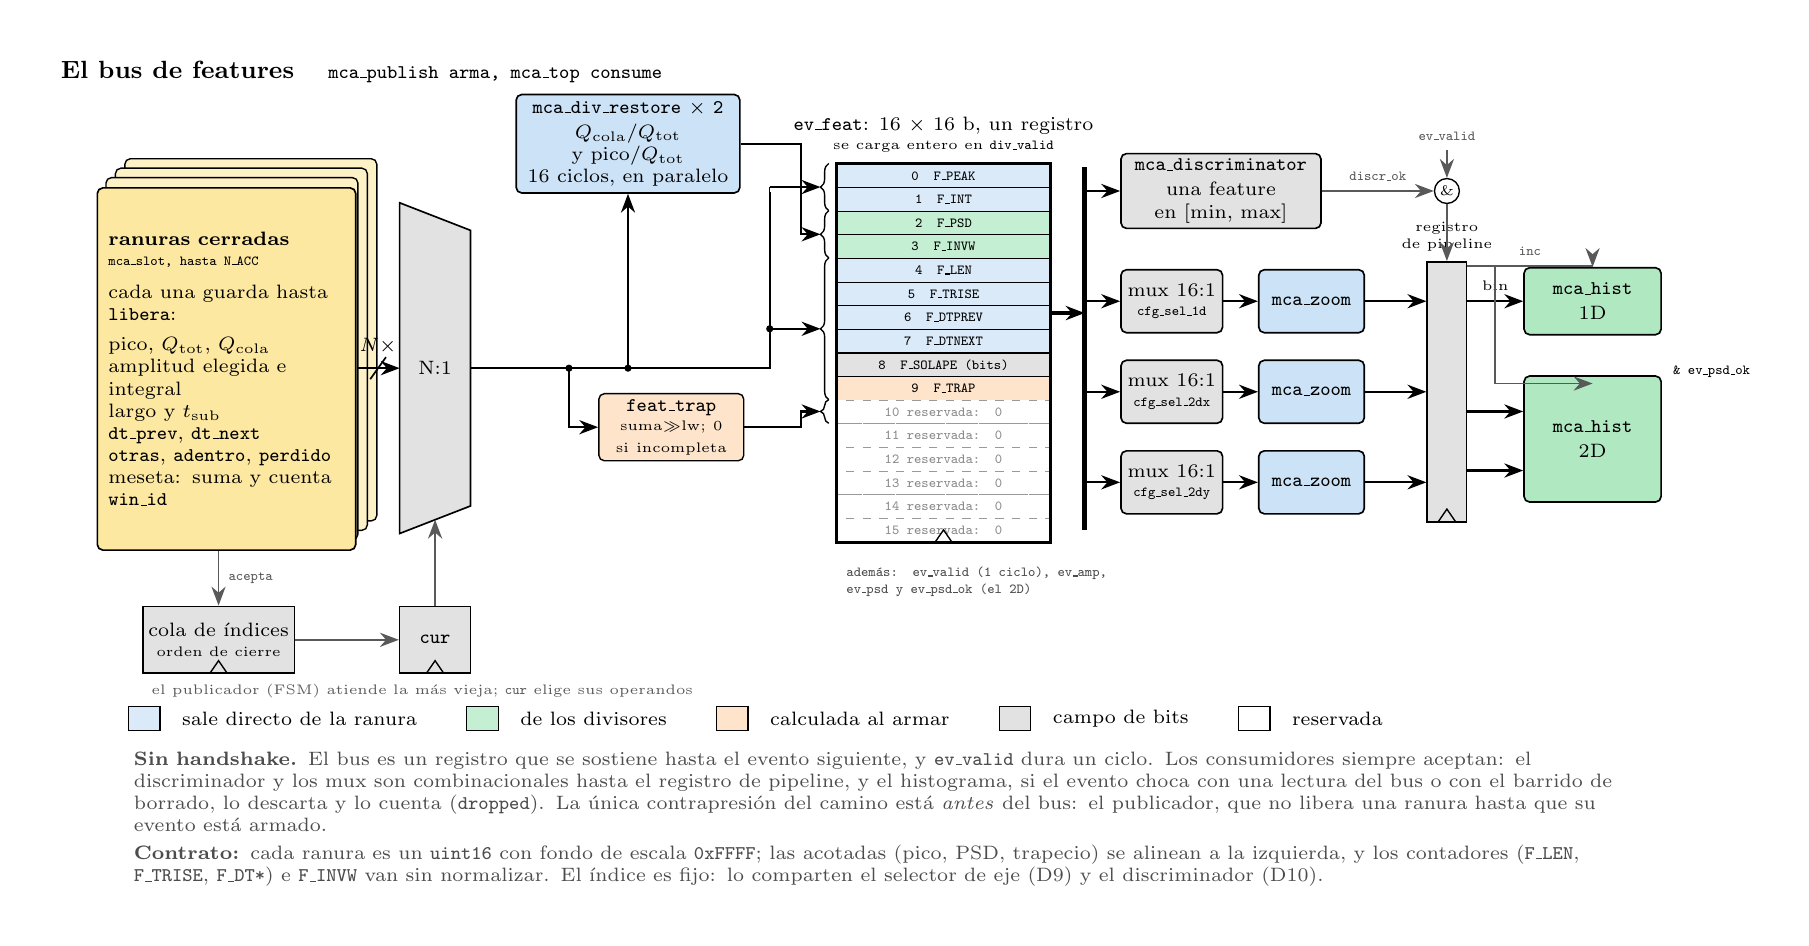
\begin{tikzpicture}[fondo]

\node[titulo] at (-0.6,1.75) {\textbf{El bus de features} \quad
  {\scriptsize\ttfamily mca\_publish arma, mca\_top consume}};

%------------------------------------------------------------------ ranuras ---
\foreach \i in {3,2,1}
  \draw[fill=amarillo!60, line width=0.5pt, rounded corners=2pt]
    (0.12*\i,0.12*\i) rectangle ++(3.2,-4.6);
\node[draw=black, fill=amarillo, line width=0.6pt, rounded corners=2pt, anchor=north west,
      text width=3.0cm, minimum height=4.6cm, minimum width=3.2cm, align=left,
      font=\scriptsize, inner sep=4pt]
  (ran) at (0,0)
  {\textbf{ranuras cerradas}\\[-1pt]{\tiny\ttfamily mca\_slot, hasta N\_ACC}\\[4pt]
   cada una guarda hasta \texttt{libera}:\\[3pt]
   pico, $Q_\mathrm{tot}$, $Q_\mathrm{cola}$\\
   amplitud elegida e integral\\
   largo y $t_\mathrm{sub}$\\
   \texttt{dt\_prev}, \texttt{dt\_next}\\
   \texttt{otras}, \texttt{adentro}, \texttt{perdido}\\
   meseta: suma y cuenta\\
   \texttt{win\_id}};

%----------------------------------------------------- la cola, cur y el mux ---
\muxdec{mx}{(4.3,-2.3)}{4.2}
\node[font=\scriptsize, align=center] at (mx) {N:1};
\draw[flujo, ancho=$N\times$] (ran.east |- mx-in) -- (mx-in);

\node[registro=1.6cm, align=center] (cola) at (1.55,-5.75)
  {cola de índices\\[-1pt]{\tiny orden de cierre}};
\node[registro=0.9cm] (cur) at (4.3,-5.75) {\texttt{cur}};
\draw[ctrl] (cola) -- (cur);
\draw[ctrl] (cur) -- (mx-sel);
\draw[ctrl] (ran.south -| 1.55,0) -- node[right, font=\tiny, align=left] {\texttt{acepta}} (cola);
\node[font=\tiny, black!65, align=left, anchor=north west] at (cola.south west)
  {el publicador (FSM) atiende la más vieja; \texttt{cur} elige sus operandos};

%--------------------------------------------------------------- divisores ---
\node[datos, text width=2.7cm, minimum height=1.25cm] (div) at (6.75,0.55)
  {\blk{mca\_div\_restore $\times$ 2}{$Q_\mathrm{cola}/Q_\mathrm{tot}$ y pico$/Q_\mathrm{tot}$\\
   16 ciclos, en paralelo}};
\node[etapa=naranja!55, text width=1.7cm, minimum height=0.75cm] (ft) at (7.3,-3.05)
  {\texttt{feat\_trap}\\[-1pt]{\tiny suma$\gg$lw; 0 si incompleta}};

%------------------------------------------------------------ los 16 carriles ---
\carril{0}{azul!25}{F\_PEAK}
\carril{1}{azul!25}{F\_INT}
\carril{2}{verde!40}{F\_PSD}
\carril{3}{verde!40}{F\_INVW}
\carril{4}{azul!25}{F\_LEN}
\carril{5}{azul!25}{F\_TRISE}
\carril{6}{azul!25}{F\_DTPREV}
\carril{7}{azul!25}{F\_DTNEXT}
\carril{8}{grisr}{F\_SOLAPE (bits)}
\carril{9}{naranja!55}{F\_TRAP}
\foreach \i in {10,...,15}
  \node[carril, fill=white, draw=black!40, dashed, text=black!45] (c\i) at (9.4,{0.3-0.3*\i}) {\i \ reservada: 0};
% el registro entero
\node[draw=black, line width=0.9pt, fit=(c0)(c15), inner sep=0pt,
      path picture={\draw[line width=0.5pt]
        ([xshift=-1.1mm]path picture bounding box.south) --
        ([yshift=1.6mm]path picture bounding box.south) --
        ([xshift=1.1mm]path picture bounding box.south);}] (bus) {};
\node[font=\scriptsize, anchor=south, align=center] at (bus.north)
  {\texttt{ev\_feat}: 16 $\times$ 16 b, un registro\\[-1pt]{\tiny se carga entero en \texttt{div\_valid}}};

% de dónde sale cada grupo: llaves a la izquierda
\draw[llave] (9.3,0.3) -- (9.3,-0.3) coordinate[midway] (g01);
\draw[llave] (9.3,-0.3) -- (9.3,-0.9) coordinate[midway] (g23);
\draw[llave] (9.3,-0.9) -- (9.3,-2.7) coordinate[midway] (g48);
\draw[llave] (9.3,-2.7) -- (9.3,-3.0) coordinate[midway] (g9);

% lo que va directo: el mux sube por una barra a las dos llaves azules
\coordinate (barra) at (8.55,0);
\draw[line width=0.8pt] (mx-out) -- (mx-out -| barra) -- (barra |- g01);
\draw[flujo, cruce] (barra |- g01) -- ([xshift=-3pt]g01);
\draw[flujo] (barra |- g48) -- ([xshift=-3pt]g48);
\fill (barra |- g48) circle (1.3pt);
% a los divisores, y de ahí a F_PSD y F_INVW
\draw[flujo] (mx-out -| div.south) -- (div.south);
\fill (mx-out -| div.south) circle (1.3pt);
\draw[flujo] (div.east) -| (8.95,0) -- (8.95,0 |- g23) -- ([xshift=-3pt]g23);
% la suma de la meseta, a F_TRAP
\draw[flujo] (mx-out -| 6.0,0) |- (ft.west);
\fill (mx-out -| 6.0,0) circle (1.3pt);
\draw[flujo] (ft.east) -- (ft.east -| 8.95,0) |- ([xshift=-3pt]g9);

% las salidas sueltas del publicador
\node[font=\tiny\ttfamily, align=left, anchor=north west, black!70] at (9.4,-4.7)
  {además: ev\_valid (1 ciclo), ev\_amp,\\ev\_psd y ev\_psd\_ok (el 2D)};

%-------------------------------------------------------------- consumidores ---
\coordinate (b) at (12.55,0);
\draw[line width=1.6pt] (b |- 0,0.25) -- (b |- 0,-4.35);
\draw[flujo, line width=1.2pt] (bus.east |- 0,-1.6) -- (b |- 0,-1.6);

\node[comp, text width=2.4cm, minimum height=0.95cm, anchor=west] (disc) at (13.0,-0.05)
  {\blk{mca\_discriminator}{una feature en [min, max]}};
\foreach \n/\s/\y in {1d/sel\_1d/-1.45, 2dx/sel\_2dx/-2.6, 2dy/sel\_2dy/-3.75} {
  \node[comp, text width=1.15cm, minimum height=0.8cm, anchor=west] (m\n) at (13.0,\y)
    {mux 16:1\\[-1pt]{\tiny\ttfamily cfg\_\s}};
  \node[datos, text width=1.2cm, minimum height=0.8cm, anchor=west] (z\n) at (14.75,\y)
    {\blk{mca\_zoom}{}};
  \draw[flujo] (m\n) -- (z\n);
}
\foreach \n in {disc, m1d, m2dx, m2dy} \draw[flujo] (b |- \n.west) -- (\n.west);

\node[registro=0.5cm, minimum height=3.3cm] (pipe) at (17.15,-2.6) {};
\node[font=\tiny, align=center, anchor=south] at (pipe.north) {registro\\de pipeline};
\foreach \n in {1d, 2dx, 2dy} \draw[flujo] (z\n) -- (z\n -| pipe.west);

\node[captura, text width=1.6cm, minimum height=0.85cm] (h1) at (19.0,-1.45)
  {\blk{mca\_hist}{1D}};
\node[captura, text width=1.6cm, minimum height=1.6cm] (h2) at (19.0,-3.2)
  {\blk{mca\_hist}{2D}};
\draw[flujo] (pipe.east |- h1) -- node[above, font=\tiny] {bin} (h1);
\draw[flujo] (pipe.east |- 0,-2.85) -- (h2.west |- 0,-2.85);
\draw[flujo] (pipe.east |- 0,-3.6) -- (h2.west |- 0,-3.6);

% inc: ev_valid y el discriminador
\node[circle, draw=black, line width=0.5pt, inner sep=1pt, font=\tiny] (y) at (17.15,-0.05) {\&};
\draw[ctrl] (disc.east) -- node[above, font=\tiny\ttfamily] {discr\_ok} (y);
\draw[ctrl] (y.north) ++(0,0.35) node[above, font=\tiny\ttfamily] {ev\_valid} -- (y.north);
\draw[ctrl] (y.south) -- (pipe.north);
\draw[ctrl] (pipe.east |- 0,-1.0) -| node[pos=0.25, above, font=\tiny\ttfamily] {inc} (h1.north);
\draw[ctrl] (pipe.east |- 0,-1.0) -- ++(0.35,0) |- ([yshift=-3pt]h2.north west) --
  ([yshift=-3pt]h2.north);
\node[font=\tiny\ttfamily, anchor=west] at (19.9,-2.35) {\& ev\_psd\_ok};

%------------------------------------------------------------------- notas ---
\leyenda{0.4,-6.75}{azul!25/sale directo de la ranura, verde!40/de los divisores,
  naranja!55/calculada al armar, grisr/campo de bits, white/reservada}
  {\textbf{Sin handshake.} El bus es un registro que se sostiene hasta el evento
   siguiente, y \texttt{ev\_valid} dura un ciclo. Los consumidores siempre aceptan:
   el discriminador y los mux son combinacionales hasta el registro de pipeline,
   y el histograma, si el evento choca con una lectura del bus o con el barrido de
   borrado, lo descarta y lo cuenta (\texttt{dropped}). La única contrapresión del
   camino está \emph{antes} del bus: el publicador, que no libera una ranura hasta
   que su evento está armado.\\[2pt]
   \textbf{Contrato:} cada ranura es un \texttt{uint16} con fondo de escala
   \texttt{0xFFFF}; las acotadas (pico, PSD, trapecio) se alinean a la izquierda, y
   los contadores (\texttt{F\_LEN}, \texttt{F\_TRISE}, \texttt{F\_DT*}) e
   \texttt{F\_INVW} van sin normalizar. El índice es fijo: lo comparten el
   selector de eje (D9) y el discriminador (D10).}

\end{tikzpicture}
\end{document}
